\section{Crear un proyecto para pruebas} 
\begin{itemize}
 \item  Crear un proyecto nuevo de C char Aplicación de consola (.NET Core) y Asigne al proyecto el nombre Bank .
\item Crear un proyecto de prueba unitaria  de prueba de MSTest (.NET Core) de C char y  Ponga al proyecto el nombre BankTests.

\begin{center}
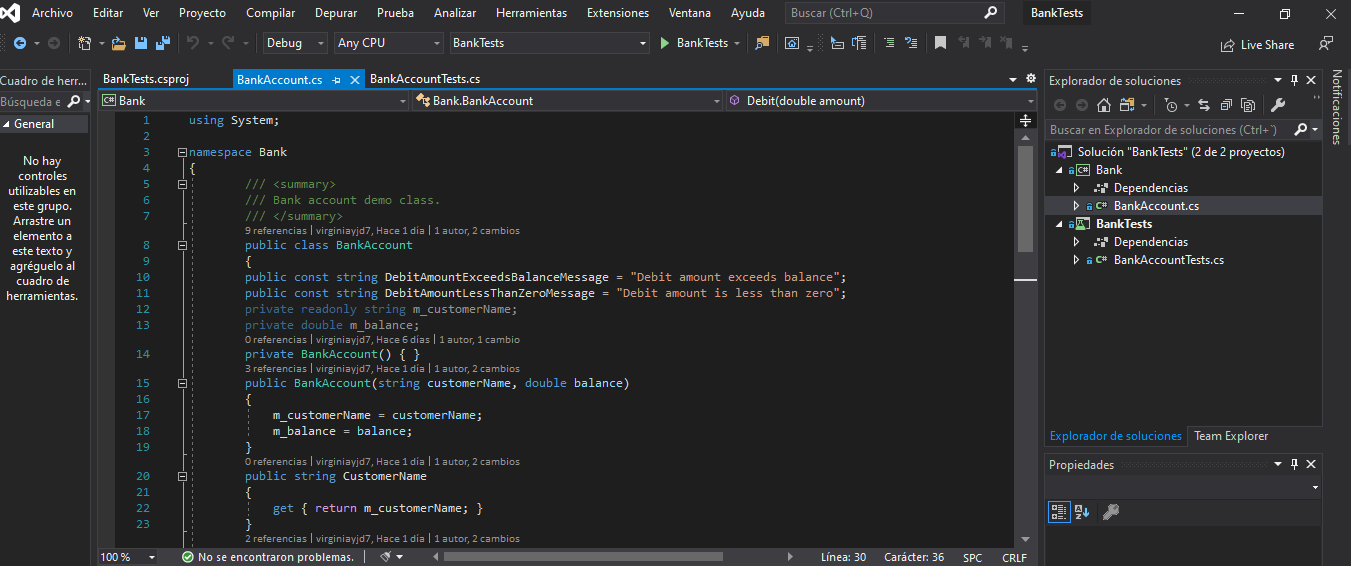
\includegraphics[width=\columnwidth]{images/1}\newline
\end{center}
\item Reemplace el contenido de Program.cs por el siguiente código de C char que define una
clase, BankAccount
\begin{center}
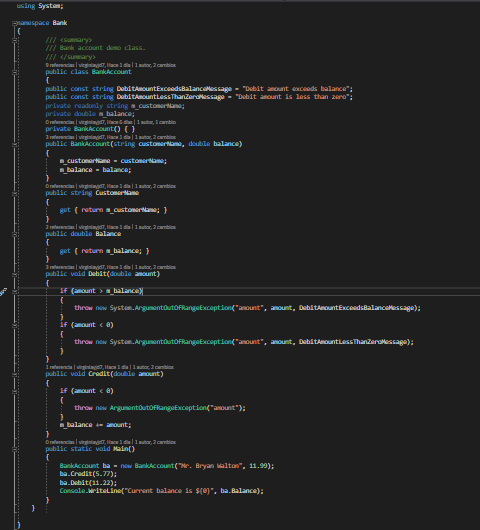
\includegraphics[width=\columnwidth]{images/2}\newline
\end{center}
\item El archivo BankAccountTests.cs contiene ahora el siguiente código:
\begin{center}
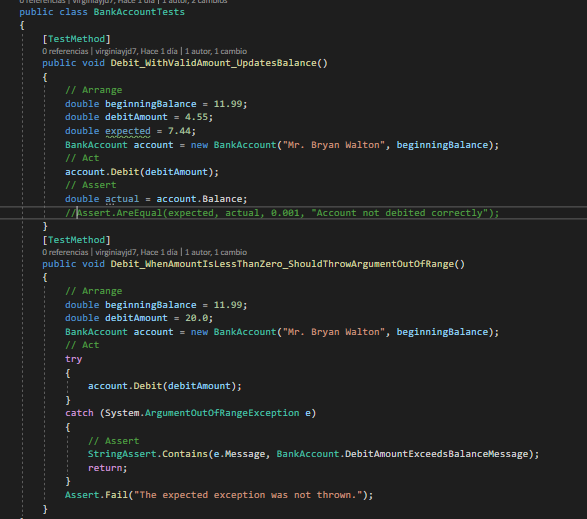
\includegraphics[width=\columnwidth]{images/3}\newline
\end{center}
\end{itemize}
\section{Resultado:Al  ejecutar la prueba, se muestra:} 
\begin{center}
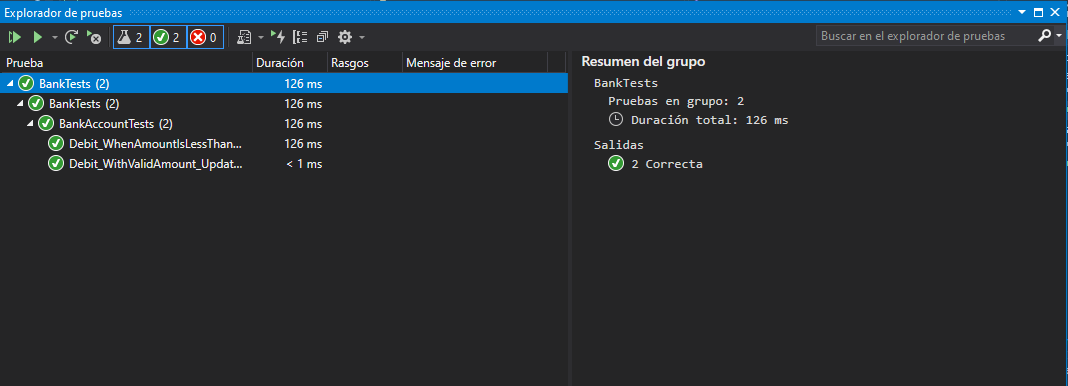
\includegraphics[width=\columnwidth]{images/final}\newline
\end{center}


